\documentclass[a4paper,12pt]{report}
\usepackage[utf8]{inputenc}
\usepackage{enumitem}
\usepackage[colorinlistoftodos]{todonotes}
\usepackage{hyperref}

\begin{document}


\chapter{Importancia de la capa de presentación en la performance}

Este capítulo esta basado en el análisis hecho por Steve Souders en \emph{``High Performance Web Sites by Steve Souders. Copyright 2007 Steve Souders,978-0-596-52930-7.''}
En el cual se realiza un estudio de la performance de varios sitios web y ciertas técnicas para   mejorarla.

\section{Investigando la performance en sitios web}

Para saber qué mejoras realizar para aumentar la performance es necesario analizar qué elementos y en qué etapas de la aplicación se consume más tiempo.
Generalmente ante un problema de performance uno de los primeros elementos a analizar es el \emph{backend} del sistema, intentando ajustar opciones del compilador,
trabajando con los índices en las bases de datos, mejorando el manejo de memoria, etc.
Analizando los resultados obtenidos luego de realizar dichas acciones sobre el \emph{backend} se puede ver que en
realidad el beneficio que representan estos cambios sobre la performance no es significativo en relación con el costo que implica su implementación.

\section{La regla de oro de la performance}

En cualquier esfuerzo por optimizar un sistema, es fundamental realizar un análisis sobre el estado actual de la performance para identificar dónde se pueden llevar a cabo
las mejoras que pueden tener mayor impacto sobre la aplicación.

Al analizar los principales sitios de Estados Unidos\todo[list]{generar gráfica con valores actuales?}, se puede ver la incidencia de la capa de presentación
en la performance, su gran potencial para mejoras y la necesidad de centrarse en ella a la hora de optimizar.

\begin{figure}[h]
\centering
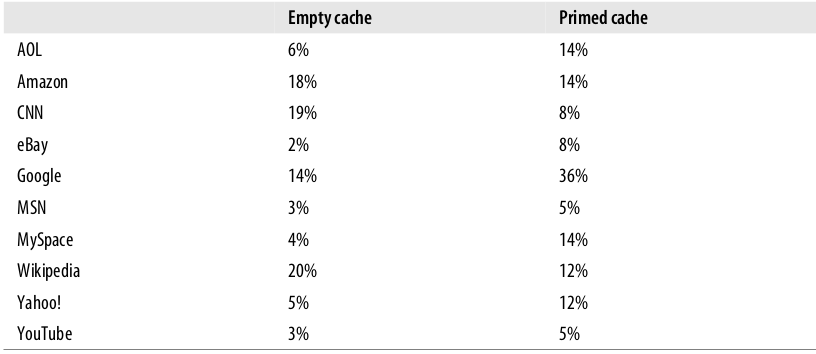
\includegraphics[width=1\textwidth]{figuras/hpws/tiempos_top10.png}
	\caption{Porcentaje de tiempo utilizado para descargar documento HTML.}
    \label{fig.tiempos_top10}
\end{figure}

Como se puede apreciar en \ref{fig.tiempos_top10} solo entre un 10 y un 20\% del tiempo de respuesta es utilizado en descargar el documento HTML, el resto
del tiempo es consumido en la capa de presentación.

Mientras que reduciendo el tiempo de respuesta del \emph{backend} a la mitad, el tiempo de respuesta del usuario se reduciría entre un 5 y un 10\%. En cambio,
si se aumenta la performance de la capa de presentación en un cincuenta por ciento, el tiempo de respuesta del usuario se reduciría entre un 40 y un 45\%.

Adicionalmente, realizar mejoras en la capa de presentación típicamente requiere menos tiempo y recursos. Generalmente mejorar el \emph{backend} involucra rediseñar la arquitectura del
programa, optimizar secciones críticas del código, incorporar hardware, distribuir bases de datos, etc. Estos proyectos pueden tardar semanas, incluso meses, en cambio la
mayoria de las mejoras que se pueden implementar para mejorar la performance de la capa de presentacion, se pueden realizar en días.

A partir de este análisis realizado sobre el estado de los principales sitios web se define la regla de oro de la performance, que indica que solamente entre un 10 y un 20\% 
del tiempo de respuesta del usuario es utilizado al descargar un documento HTML. El restante porcentaje del tiempo es utilizado en descargar los restantes
componentes en la página.

\section{Buenas prácticas para mejorar la performance de un sitio web}

\subsection{Realizar menos pedidos HTTP}

Según la \emph{Regla de oro de la performance} entre el 80 y 90\% del tiempo es utilizado para realizar pedidos HTTP de todos
los componentes referenciados en el documento HTML, desplegar imágenes y ejecutar \texttt{scripts}. Por lo tanto reduciendo el número de pedidos
HTTP se puede reducir el tiempo de respuesta.

A continuación se describen algunas técnicas para reducir el número de pedidos HTTP sin comprometer el diseño (cantidad de componentes) del sitio.
El empleo de las mismas reduce el tiempo de respuesta para todos los usuarios, pero en particular para aquellos que ingresan por primera vez al sitio y no tienen contenido
en la memoria \emph{cache} del navegador.

\subsubsection{Image Maps}

Un \texttt{image map} permite asociar varias URLs a una sola imagen. La URL de destino es elegida en base a la zona de la imagen donde el usuario realiza un \emph{click}.
Un claro ejemplo de uso de \texttt{image maps} es cuando se tiene una barra de navegación con varias imágenes, donde cada una tiene un link asociado.
En lugar de realizar un pedido HTTP por cada imagen, se realiza un solo pedido para obtener el \texttt{image map} y de esta forma se mejora el tiempo de respuesta
al reducir el numero de pedidos HTTP.

\subsubsection{CSS Sprites}

Esta técnica permite combinar varias imágenes en una sola, de forma mas flexible que los \texttt{image maps}, ya que no existe la restricción de que las imágenes
sean contiguas. Para posicionar cada imagen en el lugar correcto de la página, se utilizan las propiedades \texttt{background-image} y
\texttt{background-position} de CSS.
Al combinar las imágenes a utilizar en una única imagen se reduce la cantidad de pedidos HTTP, lo que representa una mejora en el tiempo de respuesta.

\subsubsection{Inline Images}

La técnica \emph{Inline Images} permite incluir imágenes directamente en el sitio sin realizar ningún pedido HTTP adicional al del documento HTML, pero como contrapartida
aumenta el tamaño del mismo.

Esto se logra utilizando el esquema \texttt{data: URL} definido en el rfc 2397 \cite{rfc2397}, diseñado para embeber pequeñas cantidades de datos como 
si fueran referenciados externamente.

\subsubsection{Combinar \emph{Scripts} y hojas de estilo}

Una forma de reducir el número de pedidos HTTP consiste en minimizar el número de archivos que se descargan. Generalmente los sitios web contienen
varias hojas de estilo y varios archivos de \emph{Javascript}, lo cual implica una gran cantidad de pedidos HTTP. Combinar todos los scripts en un solo archivo y
todos los CSS en una hoja de estilo reduce de manera considerable el tiempo de respuesta.

\subsection{Usar una red de Distribucion de Contenido (CDN)}

La proximidad de los usuarios al servidor web que contiene la aplicación reduce el tiempo de respuesta
de cada pedido HTTP que se realiza al servidor. Si los servidores web que contienen
los componentes de la página están próximos al usuario, los tiempos de respuesta de muchos pedidos HTTP pueden ser mejorados.

Por lo tanto, en lugar de rediseñar la aplicación distribuyendo los servidores web que contienen la aplicación, un primer paso más sencillo sería distribuir los servidores
que contienen los componentes de la página, ya que no solo se obtiene una reducción en los tiempos de respuestai, sino que también implica menores
costos y un menor esfuerzo ya que es muy simple de implementar utilizando redes de distribución de contenido.

\subsubsection{Red de Distribucion de Contenido (CDN)}

Una red de distribucion de contenido es una colección de servidores web distribuidos en diversos
lugares para entregar de forma más eficiente el contenido a los usuarios.
Los CDNs son utilizados para entregar contenido estático, imágenes, \texttt{scripts}, hojas de estilo y contenido \emph{Flash}.

La elección del servidor para hacer entrega del contenido a un usuario específico, se basa en la proximidad del usuario a la red.
Por ejemplo, el servidor elegido es el que se encuentra a menor cantidad de saltos respecto al usuario.

Además de mejorar los tiempos de respuesta, las redes de distribución de contenido brindan otros beneficios. Algunos de los servicios que incluyen son:
respaldo de información, gran capacidad de almacenamiento, \emph{caching} y absorber picos de tráfico. Una de las principales desventajas que tienen
es que los tiempos de respuesta pueden verse afectados por otros sitios, ya que las CDNs comparten sus servidores web con varios de sus clientes.

\subsection{Agregar el encabezado \texttt{Expires}}

Los sitios web contienen una gran cantidad de componentes, por lo que un usuario que visite el sitio por primera vez tendrá que realizar una gran cantidad de pedidos HTTP.
Asignando el encabezado \texttt{Expires} especificado en el rfc 2616 \cite{rfc2616} seccion 14.21, estos contenidos pueden ser almacenados en la memoria \emph{cache}
de los navegadores, lo que permite ahorrar pedidos HTTP en subsiguientes visitas al sitio.

\begin{figure}[h]
\centering
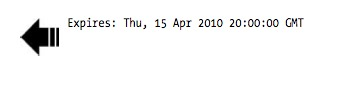
\includegraphics[width=1\textwidth]{figuras/hpws/expires.jpg}
  \caption{Ejemplo de respuesta HTTP con encabezado \texttt{Expires}.}
    \label{fig.expires}
\end{figure}

Los sevidores web utilizan el encabezado \texttt{Expires} para indicarle al cliente web que puede utilizar
la copia actual de un elemento hasta el tiempo especificado por este encabezado, como se puede apreciar en \ref{fig.expires}.
La especificación de HTTP resume este encabezado como \emph{``la fecha o tiempo después del cual es considerado como obsoleto''}.


\subsubsection{\texttt{Max-Age} y \texttt{mod\_expires}}

Una alternativa para superar las limitaciones que tiene el encabezado \texttt{Expires}, es el uso del encabezado \texttt{Cache-Control} definido en el rfc 2616 \cite{rfc2616} seccion 14.9, el cual
fue introducido en HTTP/1.1. El principal problema con \texttt{Expires} es que utiliza
una fecha específica, lo cual requiere una estricta sincronización de relojes entre el servidor y el cliente.

Por otro lado, \texttt{Cache-Control} utiliza la directiva \texttt{max-age} para especificar cuánto tiempo un componente puede ser almacenado en \emph{cache}.
Define la ventana de validez del componente en la \emph{cache} en segundos. Si desde que el componente fue pedido por primera vez transcurrieron menos de \texttt{max-age}
segundos, el navegador utilizará la versión del componente que tiene en su \emph{cache}, evitando de esta forma realizar un nuevo pedido HTTP.
El módulo \emph{mod\_expires} de Apache permite utilizar el encabezado \texttt{Expires} de forma similar a \texttt{max-age}, expresando la fecha de expiración en terminos de
años, meses, semanas, días, minutos o segundos.

\begin{figure}[h]
\centering
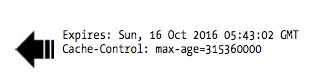
\includegraphics[width=1\textwidth]{figuras/hpws/cache-control.jpg}
  \caption{Ejemplo de respuesta HTTP con encabezado \texttt{Cache-Control}.}
    \label{fig.cache-control}
\end{figure}

Es posible tener ambos encabezados en una respuesta ya que algunos navegadores no soportan HTTP/1.1. Si los dos encabezados están presentes, la especificación
de HTTP dicta que la directiva \texttt{max-age} tiene mayor precedencia que el encabezado \texttt{Expires}.

Es común encontrar el encabezado \texttt{Expires} en imágenes, pero esta práctica debería ser aplicada a la mayoría de los componentes de un sitio. En particular
a cualquier componente que no cambie frecuentemente, incluyendo \texttt{scripts}, hojas de estilo
y componentes Flash.

\subsubsection{Renombrar archivos}

Cuando se recibe una respuesta con un encabezado \texttt{Expires}, el navegador utilizará la versión del componente que contiene en su \emph{cache} hasta
la fecha de expiración. Es por este motivo que el uso de este cabezal reduce enormemente los tiempos de respuesta. En consecuencia, por más que uno actualice un componente
en su servidor, los usuarios que ya visitaron el sitio y tienen el componente en su \emph{cache}, no obtendrán la nueva versión del mismo.

Para asegurar que los usuarios obtengan la última versión de un componente, es necesario cambiar el nombre del archivo del componente. Esta práctica es muy
sencilla si uno genera sus sitios dinámicamente utilizando lenguages como RoR, Perl, PHP, etc. Es recomendable realizar esta técnica como parte del proceso de liberación,
agregando el número de liberación a los nombres de los archivos.

\subsection{Comprimir componentes}

Esta técnica permite reducir los tiempos de respuesta al permitir generar una respuesta HTTP de menor tamaño. De esta forma, el tiempo de transferecia se ve disminuido, ya que se envía
una menor cantidad de paquetes desde el servidor hacia el cliente.

\subsubsection{Funcionamiento}

Desde que surgió HTTP/1.1, los navegadores que soportan compresión indican al servidor los tipos de compresión que soportan mediante la inclusión del encabezado
\texttt{Accept-Encoding} en el pedido HTTP. Dicho encabezado se encuentra definido en \emph{http://www.w3.org/Protocols/rfc2616/rfc2616-sec14.html sección 14.3}.

\begin{figure}[h]
\centering
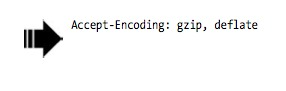
\includegraphics[width=1\textwidth]{figuras/hpws/accept-encoding.jpg}
  \caption{Ejemplo de un encabezado \texttt{Accept-Encoding}.}
    \label{fig.gzip-request}
\end{figure}

Cuando el servidor web recibe un pedido con el encabezado \texttt{Accept-Encoding}, puede comprimir la respuesta (en caso de soportarlo) utilizando alguno de los métodos listados
por el cliente en el pedido. El servidor notifica al cliente web que la respuesta esta comprimida agregando el encabezado \texttt{Content-Encoding} especificado en el rfc 2616
\cite{rfc2616} 14.11 a la respuesta HTTP.

\begin{figure}[h]
\centering
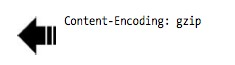
\includegraphics[width=1\textwidth]{figuras/hpws/content-encoding.jpg}
  \caption{Ejemplo de un encabezado \texttt{Content-Encoding}.}
    \label{fig.gzip-respuest}
\end{figure}

La especificación de HTTP/1.1 especifica tres métodos de compresión: \texttt{Gzip}, \texttt{deflate} y \texttt{compress}. Gzip es el más popular y efectivo, es
desarrollado por el \emph{GNU project} y se encuentra estandarizado en \emph{http://tools.ietf.org/html/rfc1952}. \texttt{Deflate} y
\texttt{Compress} especificados en el rfc \cite{rfc1950} son un poco menos efectivos y no son soportados por todos los navegadores.

\subsubsection{Qué comprimir}

Muchos sitios comprimen los documentos HTML, pero es conveniente comprimir también los \texttt{scripts} y las hojas de estilo.

La compresión tiene un costo asociado: requiere un uso adicional del CPU del lado del servidor para llevar a cabo la compresión y también del lado del cliente
para descomprimir los archivos que recibe. Para determinar si los beneficios superan a los costos de aplicar esta técnica, es necesario considerar el tamaño de la respuesta, el
ancho de banda de la conexión y la distancia entre el cliente web y el servidor. Generalmente, es útil comprimir archivos mayores a uno o dos kilobytes y no es recomendado comprimir elementos
que ya tengan alguna compresión, como imágenes o documentos PDF, ya que esto desperdiciaría el uso del CPU y podría incluso aumentar el tamaño de los archivos.

\subsection{Ubicar las hojas de estilo al comienzo}

\subsubsection{\emph{Progressive Rendering}}

Jakib Nielson deja claro en el artículo \emph{http://www.useit.com/papers/responsetime.html} la importancia del uso de indicadores de progreso.
En dicho artículo, se plantea que utilizar indicadores tiene tres ventajas: aeguran al usuario que el sistema esta en funcionamiento, indican aproximadamente cuánto tiempo el usuario debe esperar y
permiten que la espera sea menos aburrida proporcionando algo para ver.

En el caso de los sitios web, la descarga del documento HTML es el indicador de progreso. Los desarrolladores pretenden que el sitio se cargue de forma progresiva, es decir, que el
navegador despliegue contenido lo antes posible, mejorando de esta forma la experiencia de usuario. La ubicación de las hojas de estilo en el documento HTML no afecta
los tiempos de descarga, pero sí los tiempos en que el navegador despliega los elementos en la página.

El problema de posicionar las hojas de estilo al final del documento HTML es que prohíbe que los navegadores desplieguen progresivamente los componentes del sitio.
En este caso, los navegadores no despliegan elementos para evitar tener que volverlos a desplegar si su estilo cambia debido a una regla de estilo que esta definida al final del documento.

David Hyatt brinda una explicación en una serie de posts en su blog \emph{http://www.webkit.org/coding/technical-articles.html}, donde de la razón por la cual los navagadores se comportan de esta forma.
\emph{``Si los estilos todavía están cargando, es un desperdicio construir el 'rendering tree', ya que no se quiere desplegar un elemento
hasta que todos las hojas de estilo hayan sido cargadas y parseadas.''\todo[list]{como hacemos con las citas?}}

En Internet Explorer, colocar las hojas de estilo al fnal del documento causa el efecto ``Blank White Screen''. Cuando esto ocurre la página permanece completamente
en blanco hasta que en un momento todo el contenido es desplegado al unísono. Esto significa una mala experiencia de usuario, ya que no se recibe ningún
indicador de que el pedido esta siendo atendido de forma correcta.
Para evitar este efecto, es recomendable ubicar las hojas de estilo al comienzo del documento HTML, en la sección \texttt{Head} del mismo, de esta forma, los componentes
de la página se desplegarán a medida que son descargados, ya que las reglas de estilo de los mismos ya se encuentran definidas.

\subsection{Ubicar los \texttt{scripts} al final del documento HTML}

Con los \texttt{scripts} existe un problema similar al que se tiene con las hojas de estilo, pero la solución es opuesta; es mejor posicionarlos al final del documento HTML. 
De esta forma los navegadores no solo pueden desplegar progresivamente los componentes del sitio,
sino que también pueden realizar más descargas en paralelo.

\subsubsection{Problemas con \texttt{scripts}}

En la siguiente sección se describen los principales problemas que causan los \texttt{scripts} y algunas posibles soluciones.

\subsubsection{Descargas en paralelo}

El mayor impacto en el tiempo de respuesta esta determinado por el número de componentes en un sitio web, debido a que el navegador debe realizar un pedido HTTP por cada uno de ellos.
Cuando la memoria \emph{cache} del navegador se encuentra vacía, la obtención de cada componente genera un pedido HTTP. La especificación de HTTP/1.1 (rfc 2616 \cite{rfc2616} seccion 8.4)
sugiere que los navegadores pueden realizar hasta dos descargas por nombre de \emph{host} en paralelo.

Muchos sitios web descargan la mayoria de sus componentes de un sólo \emph{host}. Si un sitio web distribuye sus componentes en varios \emph{hosts}, el tiempo de respuesta
sería el doble de rápido.
Una alternativa para implementar esta técnica es utilizar \texttt{CNAMES} (DNS alias) para dividir los componentes de la página en varios \emph{hosts}.

\subsubsection{Los \texttt{scripts} bloquean las descargas}

Las descargas en paralelo se deshabilitan cuando el navegador se encuentra descargando un script, en particular el navegador no iniciará nuevas descargas, ni siquiera
desde distintos \emph{hosts}. Una de las razones de este comportamiento es que el \texttt{script} puede utilizar la función \texttt{document.write} para alterar
el contenido de la página, por lo que el navegador decide esperar para asegurarse de que la página este presentada correctamente.

Otra de las razones por las cuales las descargas en paralelo son bloqueadas mientras se descarga un \texttt{script} es para garantizar que los \texttt{scripts} sean
ejecutados en el orden correcto. Si varios \texttt{scripts} son descargados en paralelo, no existen garantías de que las respuestas de los pedidos lleguen en el
orden especificado.

\subsubsection{Ubicar los \texttt{scripts} al comienzo}

Si los \texttt{scripts} son ubicados al inicio del documento HTML, todo el contenido debajo de ellos no es renderizado y los componentes del sitio no son descargados hasta que los \texttt{scripts} son cargados. Desplegar los componentes del sitio de forma progresiva es fundamental para la experiencia del
usuario, pero los \texttt{scripts} lentos y el bloqueo de las descargas en paralelo generan una demora en la respuesta visual que el usuario recibe.

\subsubsection{Ubicar los \texttt{scripts} al final}

El mejor lugar para ubicar los \texttt{scripts} es al final del documento HTML. De esta forma no se bloquea la visualización del contenido del sitio y los elementos
que son desplegables son descargados lo mas temprano posible.

En algunos casos no es posible ubicar los \texttt{scripts} al final del documento, ya que pueden utilizar la función \texttt{document.write} para insertar parte del
contenido de la página o por problemas de \texttt{scope}. Una alternativa es utilizar \texttt{deferred} scripts. El atributo \texttt{DEFFER} indica que el \texttt{script} no
realiza una invocacion a \texttt{document.write}, y por lo tanto los navegadores pueden continuar desplegando y descargando componentes.

\subsection{Evitar \texttt{CSS Expressions}}

Las \texttt{CSS Expresions} son una forma de definir propiedades de CSS dinámicamente. Eran soportadas por Internet Explorer 5, 6 y 7, pero fueron deprecadas a
partir de Internet Explorer 8. Permiten asignar propiedades CSS como resultado de evaluaciones de codigo Javascript.

El problema con las \texttt{expressions} es que son evaluadas mas frecuentemente de lo que la gente espera. No sólo son evaluadas cuando la página es desplegada o
redimensionada, sino también cuando se avanza en la página e incluso cuando el usuario mueve el cursor sobre la misma.

\subsection{Utilizar Javascript y CSS externos}

La utilización de archivos externos de Javascript y CSS, en lugar de posicionarlos \emph{inline} generalmente produce sitios mas rápidos. Ésto se debe a que los navegadores
pueden almacenar en \emph{cache} los archivos. En caso de que los documentos HTML tengan contenido dinámico, el Javascript y el CSS \emph{inline} es descargado
cada vez que el documento HTML es pedido. En cambio, si el Javascript y el CSS se encuentran en archivos externos que se encuentran en la \emph{cache} del navegador,
el tamaño del documento HTML disminuye sin incrementar la cantidad de pedidos HTTP. El factor más importante a tener en cuenta, es la frecuencia con la cual los
archivos externos son almacenados en \emph{cache} en relación al numero de documentos HTML pedidos.

Este factor aunque es difícil de cuantificar, puede ser medido utilizando las siguientes métricas.

\subsubsection{Visitar páginas}

A menor cantidad de visitas por usuario, mayor la ventaja de utilizar \emph{inline} Javascript y CSS, ya que entre visitas, cualquier archivo externo almacenado en \emph{cache}
puede haber sido borrado de la misma. Por el contrario si el usuario típico realiza muchas visitas, es mas probable que el navegador tenga los componentes externos en su \emph{cache}.
A medida que aumentan las visitas del usuario por mes o por sesión, aumenta el beneficio de utilizar archivos externos de Javascript y CSS.

\subsubsection{Reutilización de componentes}

El uso de archivos externos permite tener una elevada tasa de reutilización de los mismos si varias páginas de un mismo sitio utilizan el mismo Javascript y CSS externo.
En caso que ninguna página comparta el mismo Javascript o CSS, la tasa de reutilización sería más baja, por lo tanto es necesario un análisis de cada sitio en
particular. Si se logra encontrar un balance que resulte en una alta tasa de reutilización, es conveniente utilizar archivos externos, en caso contrario una mejor alternativa
es tener Javascript y CSS \emph{inline}.

La única excepción donde es preferible utilizar Javascript y CSS \emph{inline} es en las paginas principales de los sitios. Esto se debe a que estas páginas
tienen un alto número de visitas, menos elementos en el \emph{cache} del navegador y una tasa de reutilización baja. Otro factor que influye en esta decisión, es la
necesidad de que el tiempo de respuesta de estas páginas sea muy reducido.

\subsubsection{Descargas \texttt{Post-Onload}}

Para las paginas principales que derivan en visitas a otras páginas del sitio, se debe utilizar Javascript y CSS \emph{inline} y precargar los archivos externos correpondientes
para las páginas secundarias. Esto se logra descargando dinámicamente los componentes externos una vez que haya terminado de cargar la pagina principal mediante
el evento \texttt{onload}. Esto hace que el navegador agregue en su \emph{cache} los archivos externos anticipando visitas del usuario a otras páginas para reducir el tiempo
de respuesta de las mismas.

\subsubsection{Dynamic Inlining}

Si un servidor pudiera saber si un componente se encuentra en el \emph{cache} del navegador, podria decidir si utilizar archivos externos es una estrategia mejor
a incluir las hojas de estilo y el codigo Javascript \emph{inline} o viceversa.
Retornando una cookie que almacena la sesion con el componente buscado, el servidor puede tomar una decisión sobre que estrategia tomar en base a la presencia o no de la
misma. En caso de que no se encuentre la \texttt{cookie} se debe utlizar Javascript y CSS \emph{inline} y en caso
contrario, se utiliza el componente externo que se encuentra en la \emph{cache} del navegador.

\subsection{Reducir las búsquedas DNS}

El \texttt{Domain Name System (DNS)} traduce nombres de \texttt{hosts} a direcciones IP. El navegador no puede descargar elementos desde un \emph{host}
hasta que se complete la búsqueda Las busquedas \texttt{DNS} tienen un costo, habitualmente toma entre veinte y cientoveinte milisegundos realizar la búsqueda de la
dirección IP de un \emph{host}. El tiempo que toma resolver la consulta depende de la proximidad que se tenga al servidor DNS, la carga que tenga el mismo y el ancho de banda
que se disponga.

\subsubsection{DNS Caching y TTLs}

Los resultados de las búsquedas de \texttt{DNS} pueden ser almacenados en \emph{cache} para mejorar la performance. Una vez que un usuario solicita la direccion IP de un \texttt{host}
el resultado de la búsqueda permanece en la memoria \emph{cache} del sistema operativo, por lo que los siguientes pedidos al mismo \texttt{host} no requieren de una nueva búsqueda.
Por otro lado los navegadores tienen su propia \emph{cache} separada del sistema operativo en la cual almacena los resultados de las busquedas \texttt{DNS}.
Mientras el navegador mantenga en su \emph{cache} el registro \texttt{DNS} no consulta al sistema operativo por dicho registro, de esta forma se reduce el timepo de busqueda.
Si el registro no se encuentra en su \emph{cache}, solicita el mismo al sistema operativo, el cual retorna el registro de su \emph{cache} (en caso de tenerlo almacenado) o
se encarga de realizar la consulta a un servidor remoto.

\subsubsection{Factores que afectan el \emph{cache} de DNS}

El servidor es el encargado de determinar cuánto tiempo deben ser almacenados en \emph{cache} los registros \texttt{DNS} mediante el valor del encabezado \texttt{TTL}.
Los navegadores por su parte, limitan el número de registros \texttt{DNS} que
mantienen en \emph{cache}, independientemente del tiempo que tengan en el mismo.
Esto se debe a que en caso que el usuario visite muchos sitios en distintos \emph{hosts} en un período corto, los registros \texttt{DNS} que se encuentran en \emph{cache}
por más tiempo son descartados para hacer lugar a los nuevos. El impacto que tiene realizar nuevamente la búsqueda de uno de los valores borrados, no es tan importante
ya que existe la posibilidad de que el sistema operativo mantenga el registro en su \emph{cache}.

Cuando el \emph{cache} del cliente (navegador y sistema operativo) no contiene registros \texttt{DNS}, la cantidad de búsquedas \texttt{DNS} es igual a la cantidad de nombres de \emph{host}
únicos en la página, esto incluye los nombres \emph{host} en la \emph{URL} de la página, imágenes, \texttt{scripts}, hojas de estilo, etc. Reducir el número de nombres de \emph{hosts}
únicos, reduce la cantidad de busquedas \texttt{DNS}, reduciendo de esta forma el tiempo de espera del usuario.
Potencialmente esto puede reducir la cantidad de descargas en paralelo que se pueden llevar a cabo, por lo tanto es necesario
encontrar un balance entre la cantidad de nombres de \emph{host} utilizados para maximizar la cantidad de descargas en paralelo y la cantidad de búsquedas \texttt{DNS} que esto tiene
como consecuencia.

\subsection{Minimizar Javascript}

\emph{Minification} es una técnica que consiste en remover caracteres innecesarios (comentarios, espacios en blanco, saltos de línea)
del código para reducir su tamaño y mejorar así el tiempo de carga, debido a que el tiempo de descarga de los archivos es menor. A medida que el uso y el tamaño de los
\texttt{scripts} y hojas de estilo aumenta, también lo hacen las ganancias obtenidas al utilizar la técnica \emph{minification}.

La ofuscación es una alternativa a la \emph{minification} que, no sólo remueve comentarios y
espacios en blanco, sino que también altera el código, reduciendo nombres de funciones y variables para que el código sea más compacto.

Mientras que la técnica \emph{Minification} es segura y sencilla, la ofuscación es bastante más compleja. Existen tres principales desventajas al ofuscar el código Javascript:
\begin{itemize}
\item \emph{Bugs}
Como la ofuscación altera el código, existe la posibilidad de introducir errores como resultado del proceso.
\item Mantenimiento
Cualquier símbolo que no debe ser modificado (nombres de funciones pertenecientes a una API) debe ser etiquetado para evitar su alteración.
\item \emph{Debugging}
Debido a que el código ofuscado es muy difícil de leer, resulta complicado depurar el código Javascript en el ambiente de producción.
\end{itemize}

\subsubsection{Evitar \texttt{redirects}}

Un \texttt{redirect} especificado en el rfc 2616 \cite{rfc2616} seccion 10.3, se utiliza para redirigir usuarios de una URL a otra. Existen diferentes motivos para realizarlo
entre ellos: redirigir a los usuarios a la nueva versión del sitio, rastrear el flujo de tráfico y crear URLs que sean fáciles
de recordar para el usuario.

Los mensajes HTTP del tipo \texttt{redirect} tienen un código de estado en el rango de los 3xx. En la especificación de HTTP 1.1, se incorporaron los códigos 303
y 307 para clarificar el uso del estado 302, pero el uso de estos últimos es casi inexistente.

\begin{figure}[h]
\centering
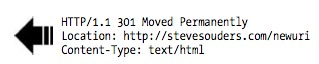
\includegraphics[width=1\textwidth]{figuras/hpws/redirect.jpg}
	\caption{Ejemplo de una respuesta con codigo de estado 301.}
    \label{fig.redirect}
\end{figure}

El navegador, al recibir un \texttt{redirect} como respuesta dirige automaticamente al usuario a la URL especificada en el encabezado \texttt{Location}
especificado en el rfc \cite{rfc2616} seccion 14.30. Toda la información necesaria para llevar a cabo el \texttt{redirect} se encuentra en los encabezados de la respuesta
y el cuerpo de la misma generalmente esta vacío. Si los encabezados \texttt{Expires}
o \texttt{Cache-Control} estan presentes en una respuesta con código 301 o 302, la misma será almacenada en el \emph{cache} del navegador.
Al insertar un \texttt{redirect} entre el usuario y el documento HTML ningún elemento de la página puede ser desplegado y ningún componente
puede comenzar a ser descargado hasta que el documento HTML haya terminado de ser descargado. Esto genera un gran atraso en la entrega del documento,
y por lo tanto en el tiempo de respuesta.

Existen otras formas para redirigir a los usuarios a otra URL. La etiqueta \texttt{refresh} incluida en la seccion \texttt{head}
 del documento HTML redirige al usuario después de un número de segundos especificado en el atritbuto \texttt{content} de la misma.
Javascript también es utilizado para realizar \texttt{redirects}, en este caso asignando la URL deseada al atributo \texttt{document.location}.

\begin{figure}[h]
\centering
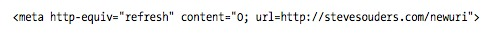
\includegraphics[width=1\textwidth]{figuras/hpws/meta-refresh.jpg}
	\caption{Ejemplo de una etiqueta refresh.}
    \label{fig.redirect}
\end{figure}

En caso que sea necesario realizar un \texttt{redirect}, la técnica recomendada por \emph{www.w3.org} es utilizar los códigos de estado 3xx de HTTP, de esta forma el
comportamiento del boton ``Atrás'' del navegador seguirá funcionando correctamente.

\subsection{Alternativas a los \texttt{redirects}}

\subsubsection{Retrobarra faltante al final de una URL}

Uno de los \texttt{redirects} más simples de evitar ocurre cuando falta una retrobarra (/) al final de una URL que la requiere. La acción de varios servidores web,
incluyendo Apache, es enviar un \texttt{redirect} cuando falta una retrobarra al final de una URL. Una forma de evitar este comportamiento en Apache es utilizar la directiva
\texttt{Alias} o el módulo mod\_rewrite.

\subsubsection{Conectar sitios web}

Frecuentemente al modificar el \texttt{backend} de un sitio web, las URLs de la nueva implementación pueden variar respecto a las originales. Una forma de dirigir a los
usuarios a la nueva URL es mediante el uso de \texttt{redirects}. A pesar de que la utilización de \texttt{redirects} reduce la complejidad para los desarrolladores, como
se mencionó previamente, el uso de esta técnica degrada la experiencia de usuario.

Las siguientes alternativas para integarar dos \texttt{backends} agregan más trabajo a los desarrolladores, pero no afectan negativamente la experiencia de usuario.
\begin{itemize}
\item
Uso de Alias, mod\_rewrite y DirectorySlash.
\item
Si los dos \emph{backends} se encuentran en el mismo servidor, el código mismo puede ser relacionado.
\item
En caso de que el dominio cambie, se puede utilizar un \texttt{CNAME} (tipo registro de DNS)  para hacer que los dos \emph{host} referencien a los
mismos servidores.
\end{itemize}

\subsection{Eliminar \texttt{scripts} duplicados}

Existen dos motivos por los cuales incluir más de una vez el mismo \texttt{script} afecta negativamente la performance: se realizan pedidos HTTP innecesarios
y se ejecuta código \emph{Javascript} innecesariamente.

Internet Explorer realiza pedidos HTTP innecesarios cuando se incluye más de una vez un \texttt{script} en un documento HTML
y el mismo no es esta especificado para ser almacenado en \emph{cache}. El navegador realiza un pedido por cada vez que este incluido el \texttt{script} en la página.
En caso que el \texttt{script} este especificado para ser almacenado en \emph{cache}, al recargar la página se realizan dos pedidos HTTP del tipo \texttt{Conditional-Get} para
confirmar que la version del elemento almacenada en el \emph{cache} sigue siendo válida.

La ejecución redundante de código Javascript sucede en todos los navegadores, independientemente si el \texttt{script} esta especificado para ser almacenado
en \emph{cache} o no, teniendo como consecuencia el uso innecesario de CPU y memoria.

Una técnica para evitar incluir el mismo \texttt{script} más de una vez es implementar un módulo de administración de \texttt{scripts}. Este modulo se encarga de incluir
\texttt{scripts} y sus dependencias si no fueron incluidos previamente.

\subsection{Configurar \texttt{ETags}}

\subsubsection{\texttt{ETags}}
\texttt{Entity Tags (ETags)} especifiacadas en el rfc \cite{rfc2616} seccion14.19, son un mecanismo utilizado por los servidores y navegadores web para verificar la validez de los componentes
que se mantienen en \emph{cache}. Una \texttt{ETag} es un string que identifica una versiÓn específica de un componente, con la restricción de que el string debe empezar
y finalizar con comillas.

\begin{figure}[h]
\centering
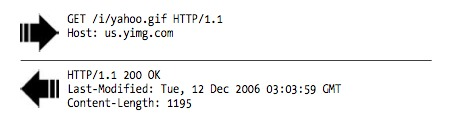
\includegraphics[width=1\textwidth]{figuras/hpws/etags.jpg}
	\caption{Ejemplo de uso de Etags.}
    \label{fig.redirect}
\end{figure}

El servidor web incluye el encabezado \texttt{ETag} en la respuesta con el string que identifica la versión del componente solicitado. Cuando el navegador realiza la
validación de la versión del componente que tiene es su \emph{cache}, envía en el pedido el encabezado \texttt{If-None-Match} con el \texttt{ETag} del componente. En caso de que
los \texttt{ETags} coincidan, el servidor responde con un mensaje con código 304 y status \texttt{Not Modified}, en caso contrario, responde con un mensaje con codigo 200
y status \texttt{OK} incluyendo la nueva versión del componente. Los \texttt{ETags} son útiles en caso de tener que validar componentes en base a una condición diferente
a la ultima fecha de modificación.

Uno de los principales problemas con las \texttt{ETags} es que son específicas para el servidor en el cual fueron creadas. En caso de utilizar un cluster de servidores para
balancear la carga de pedidos, si el navegador obtiene el componente de un servidor y después realiza un pedido condicional que es atendido por otro servidor, las
\texttt{ETags} no coincidirán, por lo tanto la segunda respuesta tiene código 200 y contiene al componente.
En caso de tener \emph{n} servidores en un cluster con una rotación del estilo \texttt{round-robin}, la probabilidad de que una \texttt{ETag} de un componente en la memoria
\emph{cache} del usuario coincida con la \texttt{ETag} correspondiente al componente en el servidor al cual se realiza el nuevo pedido es \emph{1/n}.

Las \texttt{ETags} también degradan la efectividad de los \texttt{proxy caches}. La \texttt{ETag} de un componente que mantiene un usuario en su \emph{cache} detrás de un
\emph{proxy}, generalmente no coincide con la \texttt{Etag} que mantiene en su \emph{cache} el \texttt{proxy}, teniendo como consecuencia pedidos innecesarios al servidor
original. Por lo tanto, en lugar de obtener una respuesta con código 304 entre el usuario y el \emph{proxy}, se generan dos respuestas con código 200, una entre el
servidor original y el proxy, y otra entre el \emph{proxy} y el usuario.

Otra de las desventajas de utilizar \texttt{ETags} es que el encabezado \texttt{If-None-Match} tiene precedencia sobre el encabezado \texttt{If-Modified-Since}. En caso que
se encuentren los dos encabezados en una respuesta, el servidor solo responde con un mensaje con código 304 si todos los encabezados condicionales son validos.

\subsection{Almacenar pedidos Ajax en \emph{cache}}

Uno de los principales beneficios de Ajax es que provee la posibilidad de indicarle al usuario que el sistema esta activo sin bloquear la
interfaz de usuario y permitirle al mismo seguir trabajando, al realizar pedidos al servidor web de forma asincrónica. Sin embargo, en muchas aplicaciones el
tiempo de espera del usuario se ve afectado por la forma en que se utiliza Ajax. Un factor clave que influye en el tiempo de espera del usuario, es si
los pedidos Ajax son activos o pasivos.

Los pedidos pasivos se realizan para anticipar una necesidad futura del usuario. Por ejemplo, en un cliente de correo en la web es común realizar un pedido pasivo para
obtener los contactos del usuario, para asegurar que se encuetren en el \emph{cache} para tenerlos disponibles cuando el usuario necesite escribir un correo.
Por otro lado los pedidos activos se basan en acciones del usuario. Por ejemplo listar los mensajes que cumplan con un criterio de búsqueda.

Los pedidos activos son los que tienen mayor prioridad al optimizar debido a que el usuario debe espearar a que finalicen, pero las optimizaciones a realizar, también
aplican para los pedidos pasivos. La principal mejora que se puede realizar es configurar que estos pedidos sean almacenados en \emph{cache} por el navegador, también se pueden
aplicar algunas de las técnicas ya nombradas como comprimir las respuestas, reducir las búsquedas DNS, etc.

\bibliographystyle{plain}
  \bibliography{HighPerformanceWebsites}

\listoftodos
\end{document}
